\section{TTCW Implementation with Experts as Assessors} \label{sec:data}
In this Section, we detail our implementation of creative writing evaluation using the TTCW framework derived previously. We first carefully select the 48 short stories included in the evaluation, then go over the 2.5-hour study design protocol that our 10 experiment participants followed, and finally analyze the results based on the 2,000+ individual tests administered by the experts. We leverage the collected annotations to answer the following research questions:
\begin{enumerate}[label=RQ\arabic*:,leftmargin=2.5em]
    \item \textit{Are the human-written New Yorker stories more likely to pass individual TTCW than LLM-generated stories? If so, which tests demonstrate the most significant gaps?}
    \item \textit{Is the TTCW-based creative evaluation consistent and reproducible? In other words, is there agreement among expert annotators when they perform tests for similar stories?}
    \item \textit{Which LLMs perform better in TTCW evaluation, and are there specializations observed, with some different LLMs performing better on different Torrance dimensions?}
\end{enumerate}

\subsection{Data Selection}

\begin{figure*}
\centering
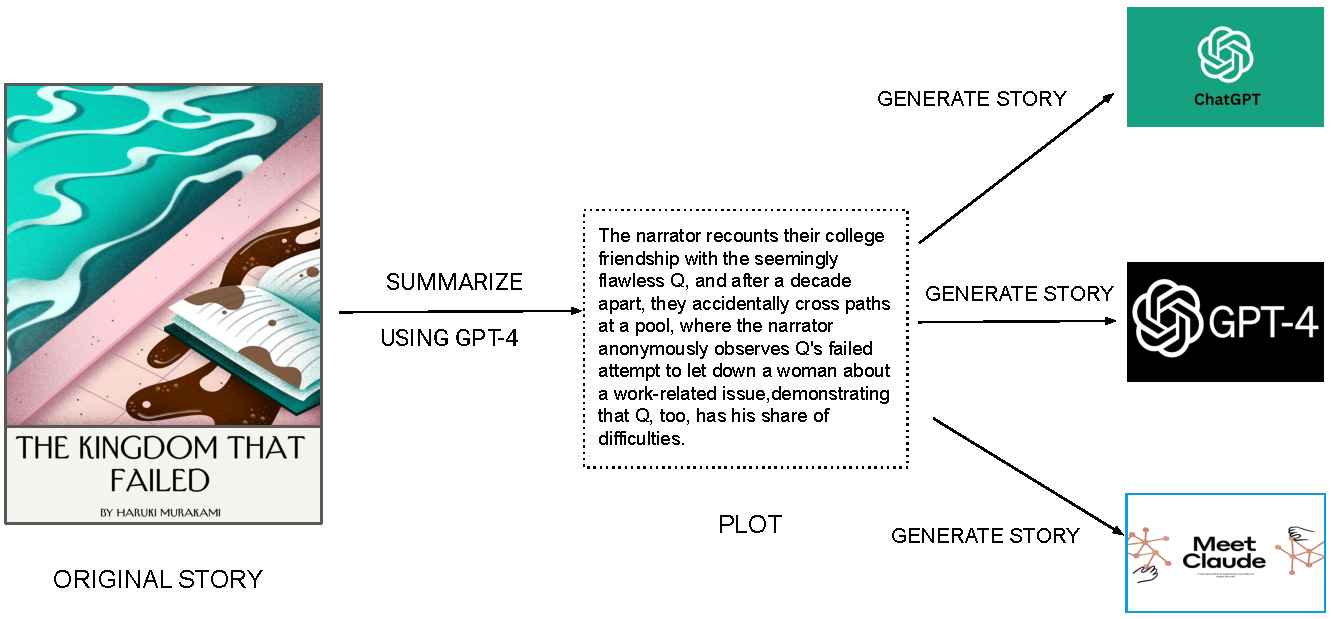
\includegraphics[width=\textwidth]{figures/datapipeline.pdf}
\caption{\label{datapipeline}Pipeline showing how our test set is created for evaluation. For each human-written original New Yorker story, we generate 3 stories from one LLM each, based on the plot of the original story. The plot is a single-sentence summary of the original story automatically generated by GPT-4 and verified by humans.}
\end{figure*}

Prior studies in the creativity of model-generated text have shown that technologies such as LLMs are capable of generative long and coherent stories \cite{yang2022doc,yang2022re3}, as well as act as assist and collaborate with creative writers \cite{yuan2022wordcraft,ippolito2022creative,mirowski2023cowriting}. For practical considerations, these studies limit their evaluation solely to model-generated content, typically only claiming relative improvements from one system to another, and do not establish whether a gap remains between high-quality human-written stories and model-generated text. Our research employs a rigorous evaluation protocol that juxtaposes human-written short stories against those constructed by LLMs to discern the potential gap, if any, in their creative quality. The dataset selection process is visually summarized in Figure~\ref{datapipeline}. We first collect 12 short stories from The New Yorker collection of short stories \footnote{https://www.newyorker.com/tag/short-stories}. Our selection criterion involved choosing short stories with diverse authors and plots. Spanning from August 13, 2020, to May 8, 2023, these stories (ranging between 1000 to 2,400 words as delineated in Figure \ref{lengthdist} in the Appendix) include compositions from acclaimed authors such as Haruki Murakami to Nobel laureate Annie Ernaux. The titles and a one-sentence plot summary (generated by GPT-4 and verified by humans) of included New Yorker short stories are listed in Table ~\ref{teststories} in Appendix.

We prompt three top-performing LLMs: GPT3.5, GPT4, and Claude V1.3 to generate a story of similar length to each New Yorker story, based on the one-sentence plot summary. We note that the choice to condition model-generated stories on the plot of the New Yorker story is an important design consideration of our evaluation. First, LLMs are known to have limited ability in devising original plotlines, as highlighted in previous research \cite{ippolito2022creative}. Second, it creates groups of stories that center around a common plot, allowing to dissociating evaluation of a story's form (i.e., creative writing), from the evaluation of plot-line creativity. 

Although LLMs were prompted to generate stories of a given length, initial experimentation by the authors of the paper revealed that the LLMs typically generate stories that can be 20-50\% more concise than intended. Length is a known confounding factor in text generation evaluation, for example with work showing that evaluators systematically prefer longer summaries as they tend to be more informative \cite{stiennon2020learning}. To address this limitation, we employed an iterative mechanism that prompted the LLM to iteratively expand on its initial story until the divergence in word count between the AI-generated and its paired human-written story was less than 200 ( See Prompt in Table \ref{promptstory} in Appendix). In our processing, all LLMs were able to converge to the desired length in at most 20 iterations. The procedure yields a total of 12 story groups, each consisting of one New Yorker story, and three LLM-generated stories, all following a common plot-line and having very similar length, for a total of 48 short stories.
We also experimented with a few other choices in prompt design such as adding \textit{You are an expert of creative fiction writing} to the beginning of the prompt or demonstrating an example New Yorker story in the prompt but these did not lead to any appreciable difference in the quality of the stories based on preliminary evaluation.

In our experiments, the stories either originate from experts or LLMs, and we do not include stories written by non-experts or `amateurs'. Although this was a consideration in the initial phases of the project, collecting amateur-written stories turned out to be a challenging and expensive process. Given the way our experiments are designed, it would require recruiting 12 non-experts to write stories given a plot since each expert-written story comes from a distinct author. The definition of an `expert' or `amateur' creative writer is difficult in a field that has unclear professional delineations. Collecting expert-written stories is straightforward as we rely on publication venue as a signal but identifying amateur writers is in itself a challenging task and might entail certain selection biases. A story written by any individual otherwise deemed as `amateur' can still be of considerable high quality. Another alternative we considered is resorting to crowd-working platforms to recruit amateurs for writing stories but a recent study by \citet{veselovsky2023artificial} highlighted the fact that approximately 33-46\% of crowd workers on such platforms currently utilize large language models (LLMs) to complete any assigned task, which would negatively impact our experiments' reproducibility. Finally adding amateur-written stories would require increased budgets for evaluation. These difficulties govern our decision not to include amateur-written stories.